\section{Methodology}
\label{sec:method}

\begin{figure}[t]
    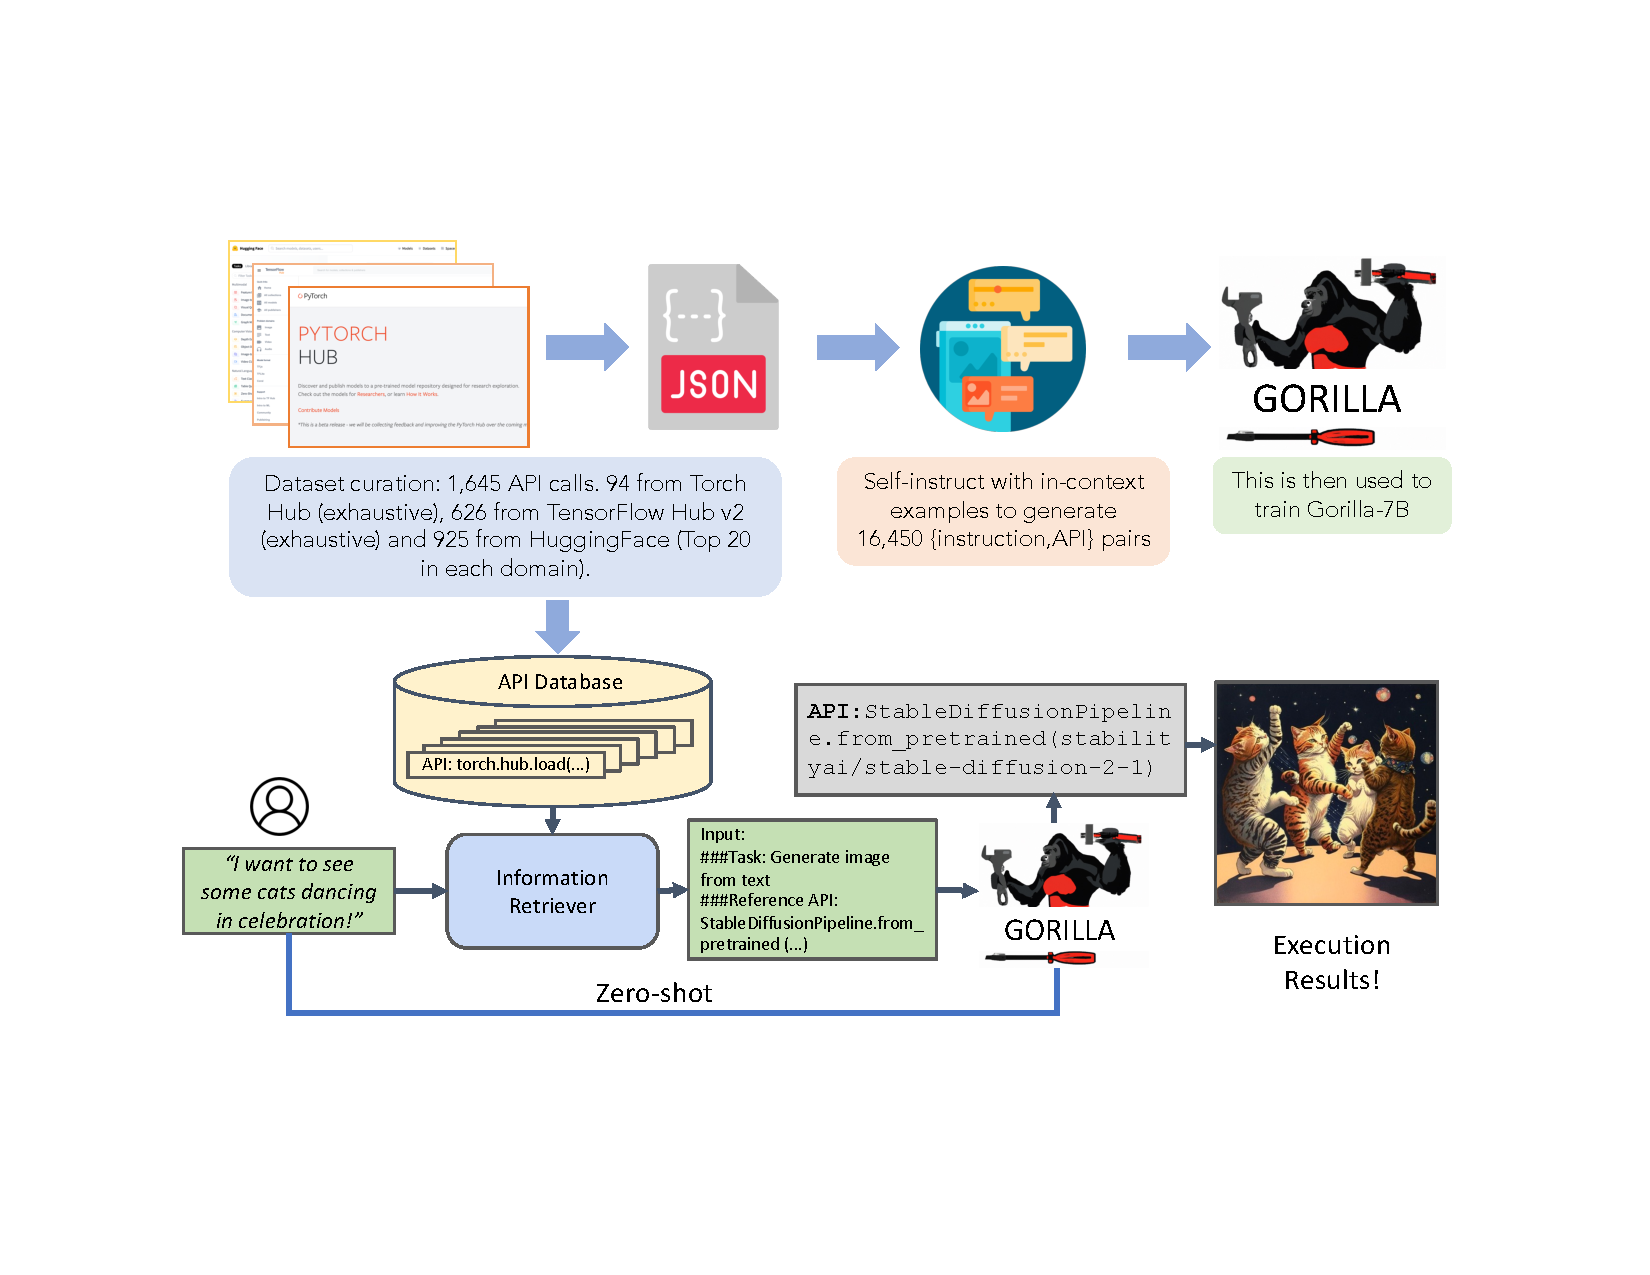
\includegraphics[width=\linewidth]{figures/llmapi.pdf}
\caption{\footnotesize \textbf{Gorilla: A system for enabling LLMs to interact with APIs.} The upper half represents the training procedure as described in Sec~\ref{sec:method}. This is the most exhaustive API data-set for ML to the best of our knowledge. During inference (lower half), \gorilla{} supports two modes - with retrieval, and zero-shot. In this example, it is able to suggest the right API call for generating the image from the user's natural language query.}
\label{fig:gorilla}
\end{figure}


In this section, we describe \oursdataset{}, a comprehensive benchmark constructed from TorchHub, TensorHub, and HuggingFace API Model Cards. We begin by outlining the process of collecting the API dataset and how we generated instruction-answer pairs. We then introduce \oursmethod{}, a novel training paradigm with a  information\---retriever incorporated into the training and inference pipelines. Finally, we present our AST tree matching evaluation metric.



\subsection{Dataset Collection}
To collect the dataset, we meticulously recorded all online model cards for HuggingFace's ``The Model Hub'', PyTorch Hub, and TensorFlow Hub Models. Throughout the rest of the paper, we call these HuggingFace, Torch Hub, and TensorFlow Hub respectively for brevity. 

\paragraph{API Documentation} The HuggingFace platform hosts and servers about 203,681 models. However, many of them have poor documentation, lack dependencies, have no information in their model card, etc. To filter these out, we pick the top 20 models from each domain. 
We consider 7 domains in multimodal data, 8 in CV, 12 in NLP, 5 in Audio, 2 in tabular data, and 2 in  reinforcement learning. Post filtering, we got a total of 925 models from HuggingFace. TensorFlow Hub is versioned into v1 and v2. The latest version (v2) has 801 models in total, and we process all of them. Post filtering out models, whose mode cards had little to no information, we are left with 626 models. Similar to TensorFlow Hub, we get 95 models from Torch Hub. 
We then converted the model cards for each of these 1,645 API calls into a json object with the following fields: \{domain, framework, functionality, api\_name, api\_call, api\_arguments, environment\_requirements, example\_code, performance, and description.\}. We provide more information in the Appendix. These fields were chose to generalize beyond the API calls within ML domain, to other domains, includin RESTful API calls. 




\paragraph{Instruction Generation}
Guided by the self-instruct paradigm~\cite{wang2022self}, we employed GPT-4 to generate synthetic instruction data. 
We provided three in-context examples, along with a reference API documentation, and tasked the model with generating real-world use cases that call upon the API. We specifically instructed the model to refrain from using any API names or hints when creating instructions. We constructed six examples (Instruction-API pairs) for each of the three model hubs. These 18 points, were the only hand-generated or modified data. For each of our 1,645 API datapoints, we sample 3 of 6 corresponding instruction examples to generate a total of 10 instruction-api pairs as demonstrated in Figure~\ref{fig:gorilla}. We would like to highlight that we only need to employ GPT-4 to generate the instructions and this can be swapped  with open-source alternatives such as LLaMA, Alpaca, etc. 

\subsection{\gorilla{}}
Our model \oursmethod{}, is retrieve-aware finetuned LLaMA-7B model, specifically for API calls. As shown in Fig~\ref{fig:gorilla}, we employ self-instruct to generate \{instruction, API\} pairs. To fine-tune LLaMA, we convert this to a user-agent chat-style conversation, where each data-point is a conversation with one round each for the user and the agent. We then perform standard instruction finetuning on the base LLaMA-7B model. For our experiments, we train \gorilla{} with and without the retriever. 

\paragraph{API Call with Constraints} API calls often come with inherent constraints. These constraints necessitate that the LLM not only comprehend the functionality of the API call but also categorize the calls according to different constraint parameters. 
This requirement introduces an additional layer of complexity to the process, demanding a more nuanced understanding from the LLM.
Specifically, for machine learning API calls, two common sets of constraints are: parameter size and a lower bound on accuracy. Consider, for instance, the following prompt: \texttt{``Invoke an image classification model that uses less than 10M parameters, but maintains an ImageNet accuracy of at least 70\%''}. Such a prompt presents a substantial challenge for the LLM to accurately interpret and respond to. Not only must the LLM understand the user's functional description, but it also needs to reason about the various constraints embedded within the request. This challenge underlines the intricate demands placed on LLMs in real-world API calls. It is not sufficient for the model to merely comprehend the basic functionality of an API call; it must also be capable of navigating the complex landscape of constraints that accompany such calls. These observations necessitate the need to fine-tune an LLM for APIs.

\paragraph{Retriever-Aware training} For training with retriever, the instruction-tuned dataset, also has an additional \texttt{"Use this API documentation for reference: <retrieved\_API\_doc\_JSON>"} appended to the user prompt. Through this, we aim to teach the LLM to parse the second half of the question to answer the first half. We demonstrate that this a) makes the LLM adapt to test-time changes in API documentation, and b) improves performance  from in-context learning, and finally c) show that it reduces hallucination error. 

Surprisingly, we find that augmenting a LLM with retrieval, does not always lead to improved performance, and can at-times hurt performance. We share more insights along with details in Sec~\ref{sec:eval}.

\paragraph{\oursmethod{} Inference} During Inference, the user provides the prompt in natural language (Fig:~\ref{fig:gorilla}). This can be for a simple task (e.g, \emph{``I would like to identify the objects in an image''}), or they can specify a vague goal, (.e.g, \emph{``I am going to the zoo, and would like to track animals''}). \gorilla{}, similar to training, can be used for inference in two modes: zero-shot and with retrieval. In zero-shot, this prompt (with NO further prompt tuning) is fed to the \gorilla{} LLM model when then returns the API call that will help in accomplishing the task and/or goal. In retrieval mode, the retriever (either of BM25 or GPT-Index) first retrieves the most up-to-date API documentation stored in the API Database. This is then concatenated to the user prompt along with the message \texttt{Use this API documentation for reference:} before feeding it to \gorilla{}.  The output of \gorilla{} is an API to be invoked. Besides the concatenation as described, we do \emph{NO} further prompt tuning in our system. While we do have a system to execute these APIs, that is not a focus of this paper. 


\subsection{Verifying APIs}

Inductive program synthesis, where a program is synthesized to satisfy test cases, has found success in several avenues~\cite{autopandas, flashfill}. 
However, test cases fall short when evaluating API calls, as it is often hard to verify the semantic correctness of the code. For example, consider the task of classifying an image. 
There are over 40 different models that can be used for the task. Even if we were to narrow down to a single family of Densenet, there are four different configurations possible. Hence, there exist multiple correct answers and it is hard to tell if the API being used is functionally equivalent to the reference API by unit tests. Thus, to evaluate the performance of our model, we compare their functional equivalence using the dataset we collected. To trace which API in the dataset is the LLM calling, we adopt the AST tree-matching strategy. Since we only consider one API call in this paper, checking if the AST of the candidate API call is a sub-tree of the reference API call reveals which API is being used in the dataset. 


Identifying and even defining hallucinations can be challenging. 
We use the AST matching process to directly identify the hallucinations. 
We define a hallucination as an API call that is not a sub-tree of any API in the database -- invoking an entirely imagined tool.
This form of hallucination is distinct from invoking an API incorrectly which we instead define as an error.


\paragraph{AST Sub-Tree Matching} We perform AST sub-tree matching to identify which API in our dataset is the LLM calling. Since each API call can have many arguments, we need to match on each of these arguments. Further, since, Python allows for default arguments, for each API, we define which arguments to match in our database. For example, we check \texttt{repo\_or\_dir} and \texttt{model} arguments in our function call. In this way, we can easily check if the argument matches the reference API or not. Please refer to Fig.~\ref{fig:ast} for more details. In this example, \gorilla{} returns a torch API call. We first build the tree, and verify that it matches a sub\-tree in our dataset along nodes \texttt{torch.hub.load}, \texttt{pytorch/vision}, and \texttt{densenet121}. But, we don't check for match along leaf node \texttt{pretrained = True} since that is an optional python argument. 


\begin{figure}[t]
    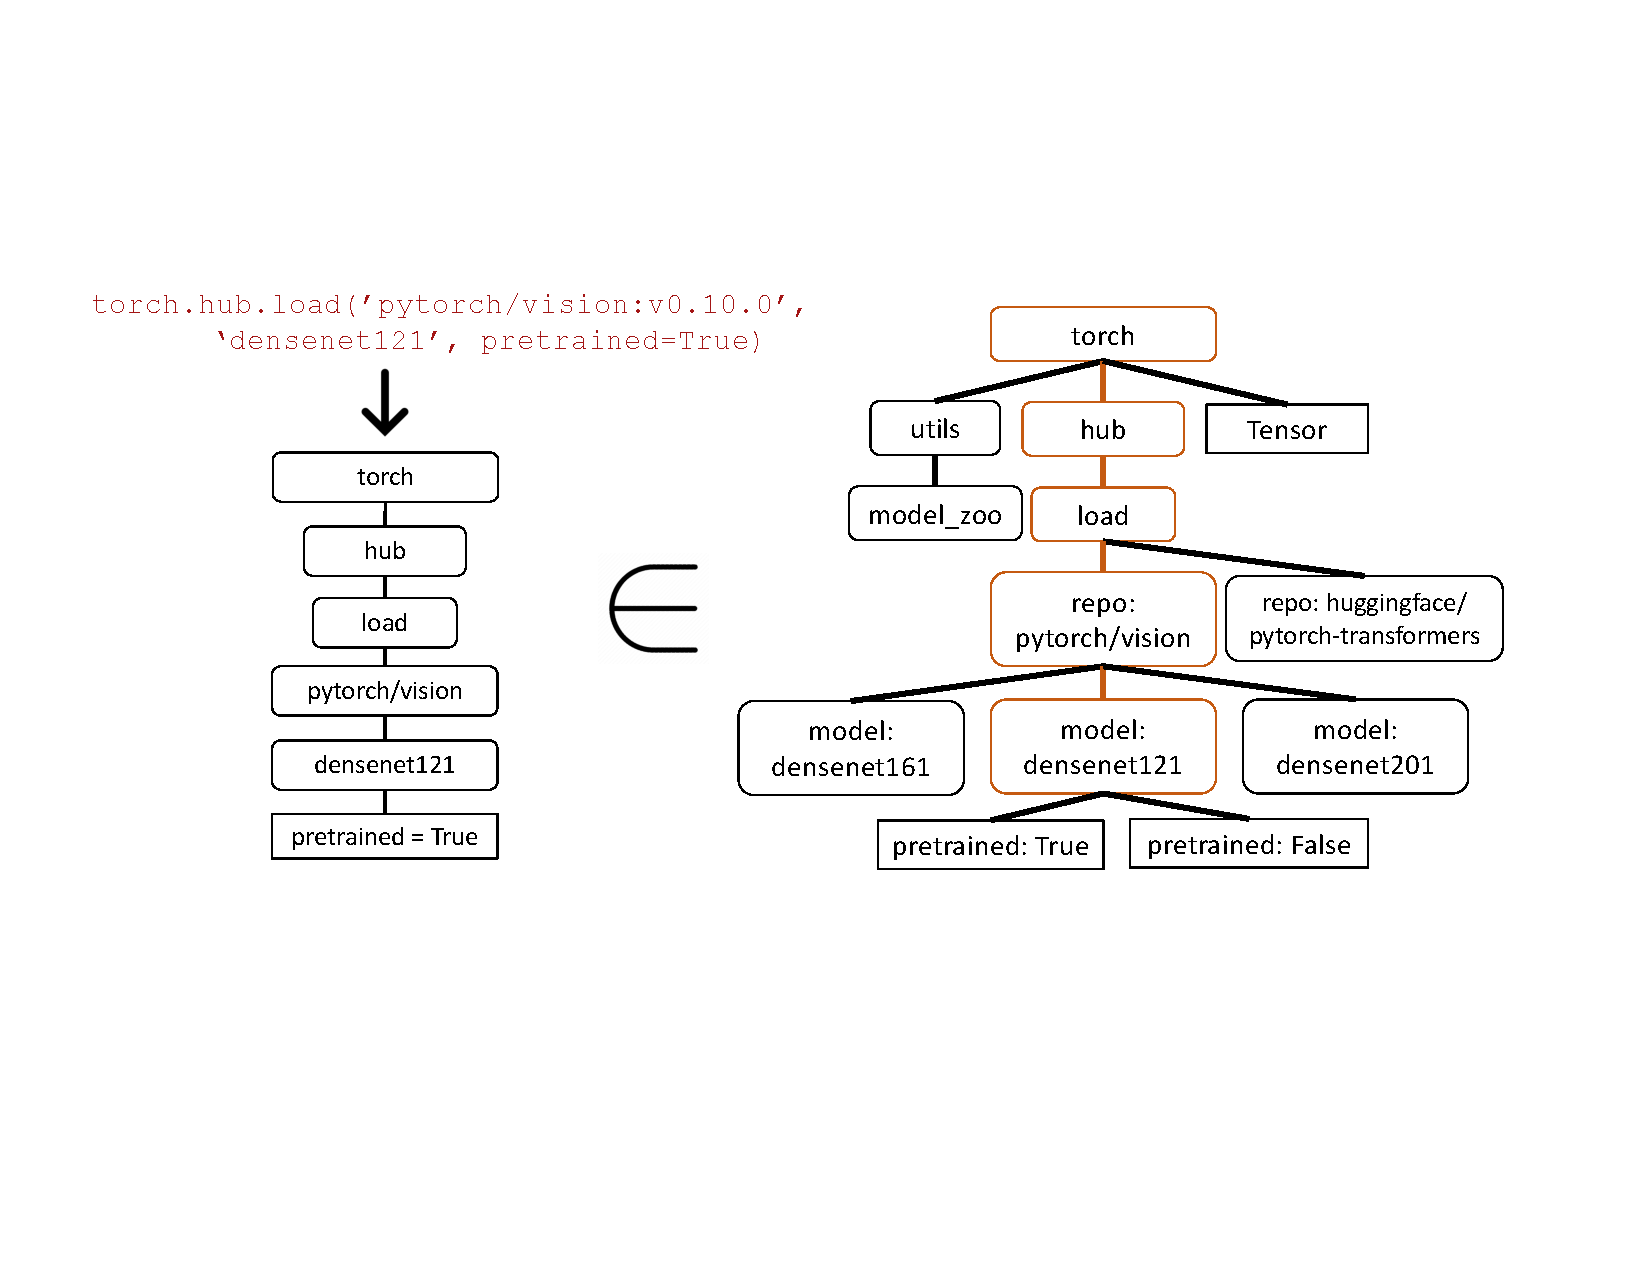
\includegraphics[width=\linewidth]{figures/ast.pdf}
\caption{\footnotesize \textbf{AST Sub-Tree Matching to evaluate API calls.} On the left is an API call returned by \gorilla{}. We first build the associated API tree. We then compare this to our dataset, to see if the API dataset has a sub\-tree match. In the above example, the matching sub\-tree is highlighted in brown, signifying that the API call is indeed correct. \texttt{Pretrained=True} is an optional argument.}
\label{fig:ast}
\end{figure}


 



